\documentclass[handout,francais]{beamer}
\usetheme{CambridgeUS}
%\input{header}
%\usepackage[utf8x]{inputenc}
\usepackage{amsmath,amsfonts,graphicx}
%\usepackage{beamerthemeONERA}
\usepackage{listings}
%\usepackage{dsfont}
%\usepackage{enumitem}
%\setlist[description]{style = multiline, labelwidth = 60pt}

\usepackage{tikz} % Required for drawing custom shapes
\usetikzlibrary{shadows, arrows, decorations.pathmorphing, fadings, shapes.arrows, positioning, calc, shapes, fit, matrix}

\usepackage{polyglossia}
%\usepackage{multirow}
%\usepackage{colortbl}

\institute
[ONERA, DTIM/CHP]
{Office National d'Etudes et de Recherches Aérospatiales,\\
\inst{1}Département Aéronautique Acoustique Aéroélasticité}


\definecolor{lightblue}{RGB}{0,200,255} 
\definecolor{paper}{RGB}{239,227,157}
\definecolor{ocre}{RGB}{243,102,25} % Define the orange color used for highlighting throughout the book
\definecolor{BurntOrange}{RGB}{238,154,0}
\definecolor{OliveGreen}{RGB}{188,238,104}
\definecolor{DarkGreen}{RGB}{0,128,0}
\definecolor{BrickRed}{RGB}{238,44,44}
\definecolor{Tan}{RGB}{210,180,140}
\definecolor{Aquamarine}{RGB}{127,255,212}
\definecolor{NavyBlue}{RGB}{0,64,128}
\definecolor{royalblue}{rgb}{0.3,0.5,0.9}
\definecolor{lightblue}{rgb}{0.7,0.7,1.0}
\definecolor{navyblue}{rgb}{0.1,0.2,0.7}
\definecolor{Maroon}{rgb}{0.5,0.5,0.1}
\definecolor{green!50!black}{rgb}{0.3,0.5,0.9}
\definecolor{darkgreen}{rgb}{0. 0.2 0}
\definecolor{darkred}{rgb}{0.4 0 0}
\definecolor{green!50!black}{rgb}{0.2 0. 0.2}
\definecolor{lightgreen!50!black}{rgb}{0.4 0. 0.4}
\definecolor{midblue}{rgb}{0. 0.2 0.4}
\definecolor{verylightgray}{rgb}{0.95 0.95 1.0}
\definecolor{lightyellow}{rgb}{1.0 0.95 0.75}


\title[Programmation des GPGPUs\hspace{2em}]{GPGPUs}
\author[Xavier JUVIGNY]{Xavier JUVIGNY}
\date{\today}

\institute{ONERA}

\begin{document}

\lstset{%
  basicstyle=\scriptsize,
  frame=single,
  keywordstyle=\color{blue},
  language=C++,
  commentstyle=\color{red},
  stringstyle=\color{brown},
  keepspaces=true,
  showspaces=false,
  tabsize=2
}

\begin{frame}
 \titlepage
\end{frame}

\begin{frame}
\frametitle{Plan du cours}
\tableofcontents
\end{frame}

\section{Architecture des GPGPUs}

\begin{frame}[fragile]{Relation CPU--GPGPU}

{\scriptsize
\begin{block}{Définition}
\begin{itemize}
\item Le GPGPU est contrôlé par le CPU comme calculateur hybride MIMD--SIMD pour exécuter
des algorithmes adaptés à son architecture;
\item CPU et GPGPU sont des calculateurs multi-c{\oe}urs et ont une mémoire architecturée sous
forme hiérarchique.
\end{itemize}
\end{block}
}

\begin{center}
\begin{tikzpicture}
\draw (-4,-2) rectangle (-1,2) (1,-2) rectangle (5,2);
\draw[fill=cyan] (-3.75,-0.5) rectangle (-1.25,1.75)
                 ( 1.25,-0.5) rectangle ( 4.75,1.75) ;
\node[color=black] at (-2.5,1.50){\scriptsize CPU multi--c{\oe}ur};
\draw[fill=orange] (-3.6,0.25) rectangle (-1.4,1.25)
                   (1.4,-0.25) rectangle (4.6,1.25);
\draw[fill=yellow] (-3.3,0.35) rectangle (-2.5,0.70)
                   (-3.3,0.80) rectangle (-2.5,1.15)
                   (-2.3,0.35) rectangle (-1.5,0.70)
                   (-2.3,0.80) rectangle (-1.5,1.15);
\node[color=black] at (-2.9,0.50){\scriptsize core 1};
\node[color=black] at (-2.9,0.97){\scriptsize core 2};
\node[color=black] at (-1.9,0.50){\scriptsize core 4};
\node[color=black] at (-1.9,0.97){\scriptsize core 3};
\draw[fill=red] (-3.6,-0.25) rectangle (-1.4,0.15);
\node[color=black] (ci) at (-2.5,-0.05){\scriptsize Internal cache};
\draw[fill=red] (-3.6,-0.65) rectangle (-1.4,-1.15);
\node[color=black] (ce) at (-2.5,-0.9){\scriptsize External cache};
\draw[fill=green] (-3.8,-1.4) rectangle (-1.2,-1.95);
\node[color=black] (me) at (-2.5,-1.65){\scriptsize RAM for CPU};
\draw[thick,blue,<->] (ci)--(ce);
\draw[thick,blue,<->] (ce)--(me);
\node[double arrow, draw, left color=blue, right color=royalblue]  at (0,-1.5){\scriptsize PCI-Express};
\node[color=black]  at (+3.0,1.50){\scriptsize GPU $n$ multi-processors};
\foreach \c in {0,0.1,0.2,0.3} {
\draw[fill=yellow]  (4.5-\c,1.1-\c) rectangle (1.8-\c,0.2-\c);
  \foreach \d in {0,0.15,0.3,...,0.9} {
    \draw[fill=Maroon]  (2.0+\d-\c,1.-\c) rectangle (2.1+\d-\c,0.7-\c);
  }
}
\node at (3.35,0.55){\scriptsize SIMD units};
\node (ml) [draw, left color=red, right color=red] at (3.0,0.1){\tiny Local memory};
\node (mgpu) [draw, left color=red, right color=red] at (3.,-1.5){\scriptsize
  RAM for GPU};
\draw[thick,blue,<->] (ml)--(mgpu);
\end{tikzpicture}
\end{center}
\end{frame}

\begin{frame}[fragile]{Détail de l'architecture GPGPU}

\begin{minipage}{55mm}
{\scriptsize
\begin{itemize}
\item GPGPU : \textcolor{orange}{Ensemble de $N$ petites unités SIMD indépendantes partageant une mémoire
global commune } : $N$ multiprocesseurs;
\item Multiprocesseur : \textcolor{orange}{Petite unité SIMD avec :}
  \begin{itemize}
    \item $k$ ALU synchronisés;
    \item 1 décodeur d'instruction;
    \item Trois mémoires partagées pour tous les ALUs (dont deux mémoires caches)
    \item R  registres distribués parmi les ALUs
      (locales à chaque \textsl{thread}) (Exemple Maxwell : 65536)
  \end{itemize}
\end{itemize}
}
\end{minipage}
\begin{minipage}{5cm}
\begin{center}
\begin{tikzpicture}
\draw[fill=cyan]   (-2cm,6cm) rectangle (2cm,1.5cm);
\draw[fill=red] (-2cm,1cm) rectangle (2cm,0.1cm);
\node at (-1.35,5.8){\tiny Device};
\node at (-0.75,0.8){\tiny Global(Device)  Memory};
\draw[fill=orange] (-1.5cm,5.5cm) rectangle (1.8cm,2.5cm);
\node at (-0.55,5.3){\tiny Multiprocessor N};
\draw[dashed,thick] (-0.55,5.2) -- (-0.75,4.6);
\draw[fill=orange] (-1.7cm,4.75cm) rectangle (1.6cm,1.75cm);
\node at (-0.75,4.5){\tiny Multiprocessor 2};
\draw[fill=orange] (-1.9cm,4.55cm) rectangle (1.4cm,1.55cm);
\node at (-0.95,4.3){\tiny Multiprocessor 1};
\draw[fill=yellow] (-1.7cm,4.1cm) rectangle (1.2cm,3.8cm);
\node at (-0.25,3.95){\tiny Local memory/L2 Cache};
\node[draw,left color=yellow, right color=yellow] at (-1.5cm,3.5cm){\tiny r};
\node[draw,left color=yellow, right color=yellow] at (-1.05cm,3.5cm){\tiny r};
\node[draw,left color=yellow, right color=yellow] at (-0.35cm,3.5cm){\tiny r};
\draw[fill=lightyellow] (-1.6cm,3.2cm) rectangle (0.3cm,3cm);
\node (p1)[draw,left color=green, right color=cyan] at (-1.45cm,3.1cm){\tiny $p_{1}$};
\node (p2)[draw,left color=green, right color=cyan] at (-1cm,3.1){\tiny $p_{2}$};
\draw[dotted,thick] (-0.75,3.1) -- (-0.25,3.1);
\node (pk)[draw,left color=green, right color=cyan] at (-0.25cm,3.1cm){\tiny
  $p_{k}$};
\node[draw,left color=green, right color=cyan] at (0.6,3.1)
{\tiny \begin{minipage}{0.7cm}Instr.\\ Unit\end{minipage}};
\draw[fill=yellow] (-1.7cm,2.7cm) rectangle (1.1cm,2.2cm);
\node at (-0.3,2.4){\tiny Texture cache};
\draw[fill=yellow] (-1.7cm,2.1cm) rectangle (1.1cm,1.6cm);
\node at (-0.3cm,1.8){\tiny Constant cache};
\draw[<->] (-1.45cm,1cm) -- (p1);
\draw[<->] (-1.00cm,1cm) -- (p2);
\draw[<->] (-0.25cm,1cm) -- (pk);
\draw[->]  (0.9cm,1cm) -- (0.9cm,1.6cm);
\draw[->]  (0.7cm,1cm) -- (0.7cm,2.2cm);
\draw[<->] (-1.3cm,3.3cm) -- (-1.3cm,3.8cm);
\draw[<->] (-0.85cm,3.3cm) -- (-0.85cm,3.8cm);
\draw[<->] (-0.1cm,3.3cm) -- (-0.1cm,3.8cm);
\draw[->]  (-1.6cm,2.7cm) -- (-1.6cm,2.9cm);
\draw[->]  (-1.15cm,2.7cm) -- (-1.15cm,2.9cm);
\draw[->]  (-0.4,2.7cm) -- (-0.4,2.9cm);
\draw[->]  (-1.3cm,2.1cm) -- (-1.3cm,2.9cm);
\draw[->]  (-0.85cm,2.1cm) -- (-0.85cm,2.9cm);
\draw[->]  (-0.1cm,2.1cm) -- (-0.1cm,2.9cm);

\node[draw,left color=blue, right color=cyan] at (0.,-1.3cm){\large CPU + RAM};
\node[double arrow, rotate=90,draw, left color=blue, right color=royalblue]  at (0,-0.5){\tiny PCI-E};

\end{tikzpicture}
\end{center}
\end{minipage}
\end{frame}

\begin{frame}[fragile]{NVIDIA : système de numérotation hardware}
\scriptsize
 \begin{block}{Numéros de version NVIDIA/Cuda}
 Deux systèmes de numérotation de version :
 \begin{enumerate}
 \item \textbf{Numérotation du hardware} : Un numéro majeur donnant l'architecture mise en {\oe}uvre sur le GPGPU utilisé, un numéro
 mineur donnant les améliorations qui ont pu y être apportées ( Exemple : parallélisme dynamique qu'à partir du hardware 3.5 ). 
 \item \textbf{Numérotation du driver} : La version de la bibliothèque Cuda utilisée ( 10.2 pour la plus récente ).
 \end{enumerate}
 \end{block}
 
 \begin{block}{Comment connaître ses numéros de version}
 \begin{enumerate}
  \item Par l'application \texttt{deviceQuery} (voir prochains transparents );
  \item En utilisant l'API C : \texttt{cudaGetDeviceProperties}
  \begin{lstlisting}
  cudaDeviceProp prop;
  cudaGetDeviceProperties(&prop, num_device);
  std::cout << "Capabilité : " << prop.major << "." 
                               << prop.minor << std::endl;
  \end{lstlisting}
 \end{enumerate}
 \end{block}
\end{frame}

\begin{frame}[fragile]{queryDevice}
 \scriptsize
 \begin{block}{Utilitaire queryDevice}
  \begin{itemize}
   \item Fourni avec les ``Samples'' proposés à l'installation par NVIDIA
   ou téléchargeables à part;
   \item Doit être compilé avant utilisation !
   \item Localisé au niveau des Samples dans \verb@1_Utilities/deviceQuery@
  \end{itemize}
 \end{block}
 
 \begin{block}{Exemple sortie obtenue ( vue partielle )}
 \begin{verbatim}
  CUDA Device Query (Runtime API) version (CUDART static linking)

Detected 1 CUDA Capable device(s)

Device 0: "GeForce GTX 970M"
  CUDA Driver Version / Runtime Version          8.0 / 8.0
  CUDA Capability Major/Minor version number:    5.2
  Total amount of global memory:                 3040 MBytes (3187343360 bytes)
  (10) Multiprocessors, (128) CUDA Cores/MP:     1280 CUDA Cores
  GPU Max Clock rate:                            1038 MHz (1.04 GHz)
  Memory Clock rate:                             2505 Mhz
  Memory Bus Width:                              192-bit
  L2 Cache Size:                                 1572864 bytes
  ...
  \end{verbatim}
 \end{block}
\end{frame}

\begin{frame}[fragile]{Organisation des c{\oe}urs de calcul}
 \begin{block}{Multiprocesseurs}
  \begin{itemize}
   \item Un GPGPU contient plusieurs multi-processeurs ( 10 dans notre exemple );
   \item Chaque multi-processeur contient une mémoire locale, des registres
   et un nombre de c{\oe}ur ( 128 dans notre exemple );
   \item Les c{\oe}urs de calcul sont organisés par groupe ( Warp ) de 16 ou
   32 threads ( selon les architectures ).
   \item Un Warp est constitué de deux demi--warps. Un demi--warp possède une architecture
   SIMD.
  \end{itemize}

 \end{block}

\end{frame}


\begin{frame}[fragile]{Organisation de la mémoire sur GPGPU}
\scriptsize
 \begin{block}{Hiérarchie mémoire}
 \begin{enumerate}
  \item Chaque thread possède sa propre mémoire locale ( registres ), éventuellement
  partagée avec les threads appartenant au même Warp.
  \item Chaque thread partage la même mémoire que les threads appartenant au même 
  ``multi--processeur'';
  \item Tous les threads partagent la même mémoire globale;
 \end{enumerate}
 \end{block}

 \begin{block}{Coalescence}
  \begin{enumerate}
   \item La mémoire globale est une mémoire entrelacée à 6 ou 12 voies ( dont deux de contrôle )
   de largeur 32 octets;
   \item Les threads d'un même warp accèdent à la mémoire globale par accès de 128 octets : une requête pour
   des données sur quatre octets, deux requêtes
   pour des données de huit octets, soit une requête par demi--warp, quatre octets pour des données de seize octets,
   soit une requête par quart de warp. 
   \item Pour cela, les données lues et écrites par un warp doivent être contiguës en mémoire et alignées sur
   128 octets.
  \end{enumerate}

 \end{block}
\end{frame}

\begin{frame}[fragile]{Coalescence}
\begin{center}
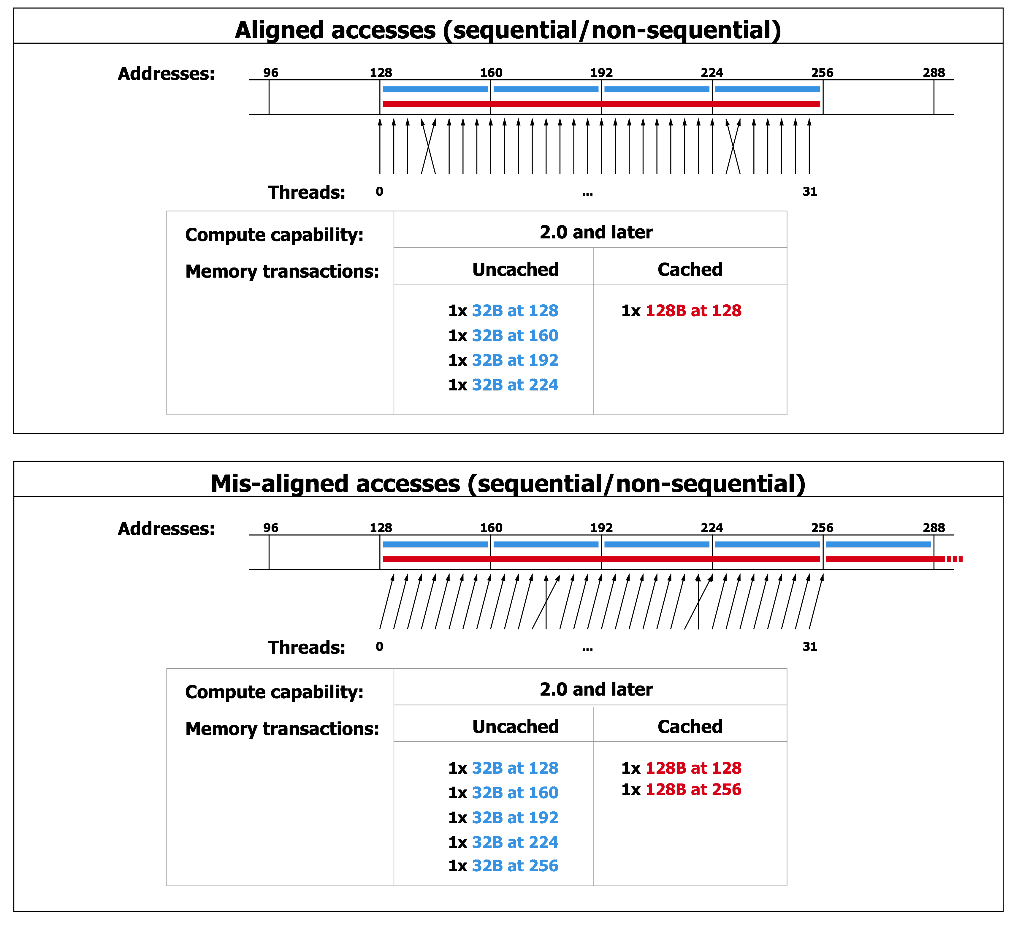
\includegraphics[width=0.7\textwidth]{Coalescence}
\end{center}
\end{frame}

\begin{frame}{Mémoire partagée}

\begin{itemize}
\item Des centaines de fois plus rapide que la mémoire globale
  \begin{itemize}
  \item 16 bancs peuvent être accédés simultanément sur
    un hardware 1.X
  \item 32 bancs peuvent être accédés simultanément sur un hardware 2.0
  \item 32 octets consécutifs sont assignés à des bancs successifs
  \end{itemize}
\item Des Threads d'un même bloc peuvent coopérer via la mémoire partagée
  \begin{itemize}
  \item 16 KBytes maximum par multiprocesseur avec un hardware 1.X 
  \item 48 KBytes maximum par multiprocesseur avec un hardware 2.0
  \item Mais sur le hardware 2.0, la mémoire cache L1 est la même mémoire que
    la mémoire partagée : le programmeur doit contrôler la taille de mémoire utilisée
    par le cache L1 et la mémoire partagée.
  \end{itemize}
\item Permet d'éviter des accès non coalescent en mémoire globale  
\end{itemize}
\end{frame}

\begin{frame}{Mémoire partagée : problèmes de performance }

\begin{itemize}
\item Les cas idéaux :
  \begin{itemize}
  \item Si tous les threads d'un demi-warp (ou un warp pour le hardware 2.0)
    accèdent à des bancs différents, pas de conflit de bancs
  \item Si tous les threads d'un demi-warp (un warp en 2.0) lisent une adresse
    identique, pas de conflit de bancs (broadcast)
  \end{itemize}
\item Les pires cas :
  \begin{itemize}
  \item Conflit de banc  : Plusieurs threads d'un même (1/2)-warp accèdent à un même banc
  \item L'accès est sérialisé
  \item Coût = max \# d'accès simultanés à un même banc
  \end{itemize}
\end{itemize}
\end{frame}

\begin{frame}{Accès à la mémoire partagée}

\begin{minipage}[c]{3cm}
\begin{tikzpicture}
\draw[xstep=1cm,ystep=0.5cm] (0,0) grid (1cm,8cm);
\draw[xstep=1cm,ystep=0.5cm] (1.99cm,0) grid (3cm,8cm);
\foreach \b / \x in {0 / 0.25,1 / 0.75,2 / 1.25, 3/1.75, 4/2.25,
  5/2.75, 6/3.25, 7/3.75, 8/4.25, 9/4.75, 10/5.25, 11/5.75,
  12/6.25, 13/6.75, 14/7.25,15 / 7.75} {
\draw (0.5cm,\x cm) node {\tiny Thread \b};
\draw (2.5cm,\x cm) node {\tiny Bank   \b};
\draw[thick, color=blue,->] (1cm, \x cm) -- (2cm, \x cm);
}
\end{tikzpicture}
\end{minipage}
\begin{minipage}[c]{4cm}
\small
\textbf{Motif d'accès sans conflits de bancs} :
chaque thread du demi-warp accède à un banc différent.
\end{minipage}
\begin{minipage}[c]{3cm}
\begin{tikzpicture}
\draw[xstep=1cm,ystep=0.5cm] (0,0) grid (1cm,8cm);
\draw[xstep=1cm,ystep=0.5cm] (1.99cm,0) grid (3cm,8cm);
\foreach \b / \x in {0 / 0.25,1 / 0.75,2 / 1.25, 3/1.75, 4/2.25,
  5/2.75, 6/3.25, 7/3.75, 8/4.25, 9/4.75, 10/5.25, 11/5.75,
  12/6.25, 13/6.75, 14/7.25,15 / 7.75} {
\draw (0.5cm,\x cm) node {\tiny Thread \b};
\draw (2.5cm,\x cm) node {\tiny Bank   \b};
}
\foreach \b / \x in {0.25 / 1.25,0.75 / 0.25,1.25 / 2.75, 1.75/1.75, 2.25/2.25,
  2.75/0.75, 3.25/3.25, 3.75/3.75, 4.25/5.75, 4.75/4.75, 5.25/5.25, 5.75/4.25,
  6.25/6.25, 6.75/6.75, 7.25/7.25,7.75 / 7.75} {
\draw[thick, color=blue,->] (1cm, \b cm) -- (2cm, \x cm);
}
\end{tikzpicture}
\end{minipage}
\end{frame}

\begin{frame}{Accès mémoire partagée}

\begin{minipage}[c]{3cm}
\begin{tikzpicture}
\draw[xstep=1cm,ystep=0.5cm] (0,0) grid (1cm,8cm);
\draw[xstep=1cm,ystep=0.5cm] (1.99cm,0) grid (3cm,8cm);
\foreach \b / \x in {0 / 0.25,1 / 0.75,2 / 1.25, 3/1.75, 4/2.25,
  5/2.75, 6/3.25, 7/3.75, 8/4.25, 9/4.75, 10/5.25, 11/5.75,
  12/6.25, 13/6.75, 14/7.25,15 / 7.75} {
\draw (0.5cm,\x cm) node {\tiny Thread \b};
\draw (2.5cm,\x cm) node {\tiny Bank   \b};
\draw[thick, color=blue,->] (1cm, \x cm) -- (2cm, 4.75 cm);
}
\end{tikzpicture}
\end{minipage}
\begin{minipage}[c]{4cm}
\small
\begin{itemize}
\item[$\leftarrow$] Chaque thread lit une adresse d'un même banc : pas de conflit
  (broadcasting)
\item[] Plusieurs Threads accèdent au même banc : \alert{conflit $\rightarrow$}
\end{itemize}
\end{minipage}
\begin{minipage}[c]{3cm}
\begin{tikzpicture}
\draw[xstep=1cm,ystep=0.5cm] (0,0) grid (1cm,8cm);
\draw[xstep=1cm,ystep=0.5cm] (1.99cm,0) grid (3cm,8cm);
\foreach \b / \x in {0 / 0.25,1 / 0.75,2 / 1.25, 3/1.75, 4/2.25,
  5/2.75, 6/3.25, 7/3.75, 8/4.25, 9/4.75, 10/5.25, 11/5.75,
  12/6.25, 13/6.75, 14/7.25,15 / 7.75} {
\draw (0.5cm,\x cm) node {\tiny Thread \b};
\draw (2.5cm,\x cm) node {\tiny Bank   \b};
}
\foreach \b / \x in {0.25 / 1.25,0.75 / 0.25,1.25 / 1.75, 1.75/1.75, 2.25/2.25,
  2.75/0.75, 3.25/3.25, 3.75/3.25, 4.25/3.25, 4.75/4.75, 5.25/5.25, 5.75/4.25,
  6.25/6.25, 6.75/6.75, 7.25/7.25,7.75 / 7.75} {
\draw[thick, color=red,->] (1cm, \b cm) -- (2cm, \x cm);
}
\end{tikzpicture}
\end{minipage}
\end{frame}

\section{Modèle de programmation}

\subsection{Outils de compilation}

\begin{frame}[fragile]{Principe de compilation CUDA et C++}
 Plusieurs cas de figure :

\begin{itemize}
\item Compilation d'un code entièrement développé en CUDA;
\item Compilation d'un code CUDA avec récupération de code C/C++;
\item Compilation code CUDA avec compilateur spécifique pour 
  la partie C/C++ sur CPU.
\end{itemize}

\end{frame}



\begin{frame}{Compilation d'un code entièrement développé en CUDA}

  \begin{exampleblock}{Contenu et production du code}
    \begin{itemize}
    \item Définitions variables et fonctions avec ``qualificateurs''
      CUDA.
    \item Du code C ou C++ avec fonctionnalités CUDA;
    \item Code C ou C++ ``standard''.
    \item Les extensions : ``.h'' pour les headers, ``.cu'' pour les sources.
    \item On compile à l'aide du compilateur NVidia : \texttt{nvcc}
    \item On obtient un code CPU contenant du code GPU intégré.
    \end{itemize}
  \end{exampleblock}

  \begin{alertblock}{Pour les codes C/C++ simples}
    \begin{itemize}
    \item Possibilité de tout compiler avec nvcc dans des fichiers .cu
    \item Mais les optimisations pour le CPU peuvent en souffrir.
    \end{itemize}
  \end{alertblock}
\end{frame}

\begin{frame}{Compilation d'un code avec récupération sources C/C++}
  \begin{exampleblock}{Contenu et production du code}
    \begin{itemize}
    \item On compile les fichiers C/C++ (.c, .cc, .h)  avec nvcc;
    \item Les fichiers contenant du code Cuda (.cu, .h) avec nvcc;
    \item On fait une édition des liens du tout pour obtenir un code binaire
      contenant les binaires pour le CPU et le GPU.
    \end{itemize}
  \end{exampleblock}

  \begin{alertblock}{Problèmes}
    \begin{itemize}
  \item A l'édition des liens, des problèmes peuvent apparaître avec des templates\ldots
  \item Problèmes d'optimisations pour le code CPU pouvant apparaître.
    \end{itemize}
  \end{alertblock}
\end{frame}

\begin{frame}{Compilation d'applications CUDA avec compilateur spécifique}

  \begin{exampleblock}{Contenu et production du code}
    \begin{itemize}
    \item Codes  C/C++ (.c, .cc, .h) : On le compile avec son
      compilateur préféré (gcc, g++, icc, \ldots);
    \item Code Cuda : On le compile avec nvcc;
    \item On fait l'édition de lien des objets obtenus
    \end{itemize}
  \end{exampleblock}

  \begin{alertblock}{Problèmes}
    \begin{itemize}
    \item Des problèmes de nommage peuvent apparaître (mais pas avec
      \textbf{gcc}).
    \end{itemize}
  \end{alertblock}
\end{frame}

\begin{frame}{Principe d'exécution}
\begin{exampleblock}{Exécution d'une application CUDA}
\begin{itemize}
\item On lance une application CPU d'apparence classique;
\item On réalise du ``Remote Process Control'' (RPC) sur le GPU depuis le CPU
(exécution de ``kernels'');
\item Pour être efficace, il faut minimiser les transferts des données;
\item On peut exécuter les ``kernels'' en mode bloquant (synchrone) ou 
  non bloquant (asynchrone) pour le programme CPU :
  $\rightarrow$ possibilité d'utiliser simultanément le CPU et le GPU.
\end{itemize}
\end{exampleblock}


\end{frame}

\subsection{Programmation des noyaux}

\begin{frame}[containsverbatim]{C étendu}
\scriptsize
  \begin{itemize}
  \item \textbf{\textcolor{blue}{Nouv. déclarations}} : \textcolor{orange}{\small global, device, shared, local, constant}
    \begin{lstlisting}
      __device__ float filter[N];
      __global__ void  convolve(float* image) {
      __shared__ float region[M];
    \end{lstlisting}
  \item \textbf{\textcolor{blue}{nouveaux mots clefs}} : 
    \textcolor{orange}{\small threadIdx, blockIdx}
    \begin{lstlisting}
      region[threadIdx] = image[i];
    \end{lstlisting}
  \item \textbf{\textcolor{blue}{Intrinsics}} : 
    \textcolor{orange}{\small \_\_syncthreads}
    \begin{lstlisting}
      __syncthreads(); image[j] = result;
  \end{lstlisting}
  \item \textbf{\textcolor{blue}{API d'exécution}} :
    \textcolor{orange}{\small Memory, symbol, execution management}
    \begin{lstlisting}
      void* myImg = cudaMalloc(bytes);// Alloue memoire sur GPU
    \end{lstlisting}
  \item \textcolor{blue}{\bf Exécution de fonction}
    \begin{lstlisting}
      convolve<<<100,10>>>(myImg);// 100 blocs de 10 threads
    \end{lstlisting}
  \end{itemize}
\end{frame}

\begin{frame}{``Qualifieurs'' de CUDA}

\underline{Propriétés des ``qualifieurs'' de CUDA}:
{\scriptsize
  \begin{tabular}{c|ccc}
    & \textcolor{blue}{\small\texttt{\_\_device\_\_}}
    & \textcolor{blue}{\small\texttt{\_\_host\_\_}}  
    & \textcolor{red}{\small\texttt{\_\_global\_\_}} \\[3mm]
    Fonctions & 
    \begin{minipage}{25mm}
      Appel sur \textcolor{orange}{GPU} \\
      Exécution sur \textcolor{orange}{GPU}
    \end{minipage} &
    \begin{minipage}{25mm}
      Appel sur \textcolor{blue}{CPU} \\
      Exécution sur \textcolor{blue}{CPU}
    \end{minipage} &
    \begin{minipage}{25mm}
      Appel sur \textcolor{blue}{CPU} \\
      Exécution sur \textcolor{orange}{GPU}
    \end{minipage} \\[2mm] \hline
  & \textcolor{red}{\small\texttt{\_\_device\_\_}} &
    \textcolor{blue}{\small\texttt{\_\_constant\_\_}} &
    \textcolor{red}{\small\texttt{\_\_shared\_\_}} \\[3mm]
  & \begin{minipage}{25mm}
      Mémoire globale \textcolor{orange}{GPU}
    \end{minipage}&
    \begin{minipage}{25mm}
      Mémoire constante \textcolor{orange}{GPU}
    \end{minipage} &
    \begin{minipage}{25mm}
      Mémoire partagé multi-processeurs
    \end{minipage} \\[5mm]
    Variables & 
    \begin{minipage}{25mm}
      Temps de vie de l'application
    \end{minipage} &
    \begin{minipage}{25mm}
      Temps de vie de l'application
    \end{minipage} &
    \begin{minipage}{25mm}
      Temps de vie du bloc de thread
    \end{minipage} \\[5mm]
    & \begin{minipage}{25mm}
      Lisible/enregistrable sur \textcolor{blue}{CPU} et \textcolor{orange}{GPU}
    \end{minipage} &
    \begin{minipage}{25mm}
      Enregistrable \textcolor{blue}{CPU}, lisible \textcolor{orange}{GPU}
    \end{minipage} &
    \begin{minipage}{25mm}
      Lisible sur \textcolor{orange}{GPU} : utilisé comme \textsl{cache} mémoire géré à la main
      pour la mémoire global \textcolor{orange}{GPU}
    \end{minipage}
  \end{tabular}
}

$\rightarrow$ Les qualifieurs séparent les codes \textcolor{blue}{CPU} et \textcolor{orange}{GPU}.
\end{frame}

\begin{frame}[containsverbatim]{Distribution des threads : grilles et blocs}
\scriptsize
\begin{minipage}[c]{52mm}
\begin{itemize}
\item Un noyau est exécuté comme une grille de blocs de thread
  \begin{itemize}
  \item 
    \textcolor{orange}{\scriptsize Tous les threads partagent le même espace de mémoire de donné}
  \end{itemize}
\item Un bloc de threads est un ensemble de threads qui peuvent coopérer les uns les autres en :
  \begin{itemize}
  \item \textcolor{orange}{\scriptsize synchronisant leur exécution}
  \item \textcolor{orange}{\scriptsize partageant leurs données à travers une mémoire partagée rapide}
  \end{itemize}
\item Deux threads provenant de deux blocs différent ne peuvent pas coopérer :
  \begin{itemize}
  \item 
  \textcolor{orange}{\scriptsize Opérations atomiques}
\end{itemize}
\end{itemize}
\end{minipage}
\begin{minipage}[c]{53mm}
\begin{tikzpicture}{56mm}
\draw[fill=cyan] (0,0) rectangle (1cm,7cm);
\node[color=black] at (2.5mm,68mm){\tiny \textbf{Host}};
\draw[fill=green] (6mm,50mm) node[draw,fill] (K1) {\tiny
  \begin{minipage}{6mm}Kernel\\ 1\end{minipage}};
\draw[fill=green] (6mm,30mm) node[draw,fill] (K2) {\tiny
  \begin{minipage}{6mm}Kernel\\ 2\end{minipage}};
\draw[color=white,->,thick] (1mm,60mm) -- (1mm,1mm);

\draw[fill=cyan] (15mm,0mm) rectangle (5cm,7cm);
\node at (20mm,68mm){\tiny \textbf{device}};
\draw[fill=green] (17mm,41mm) rectangle (48mm,65mm);
\node at (25mm,62mm){\tiny \textbf{Grid 1}};
\draw[fill=yellow] (22mm,55mm) node[draw,fill] (B00) {\tiny
  \begin{minipage}{6mm}Block\\(0,0)\end{minipage}};
\draw[fill=yellow] (32mm,55mm) node[draw,fill] (B10) {\tiny
  \begin{minipage}{6mm}Block\\(1,0)\end{minipage}};
\draw[fill=yellow] (42mm,55mm) node[draw,fill] (B20) {\tiny
  \begin{minipage}{6mm}Block\\(2,0)\end{minipage}};

\draw[fill=yellow] (22mm,46mm) node[draw,fill] (B01) {\tiny
  \begin{minipage}{6mm}Block\\(0,1)\end{minipage}};
\draw[fill=yellow] (32mm,46mm) node[draw,fill] (B11) {\tiny
  \begin{minipage}{6mm}Block\\(1,1)\end{minipage}};
\draw[fill=yellow] (42mm,46mm) node[draw,fill] (B21) {\tiny
  \begin{minipage}{6mm}Block\\(2,1)\end{minipage}};
\draw[thick, ->] (K1) -- (17mm,50mm);


\draw[fill=green] (21mm,11mm) rectangle (44mm,40mm);
\node at (29mm,38mm){\tiny \textbf{Grid 2}};

\draw[fill=yellow] (26mm,30mm) node[draw,fill] {\tiny
  \begin{minipage}{6mm}Block\\(0,0)\end{minipage}};
\draw[fill=yellow] (36mm,30mm) node[draw,fill] {\tiny
  \begin{minipage}{6mm}Block\\(1,0)\end{minipage}};
\draw[thick,->] (K2) -- (21mm,30mm);

\draw[thick,dashed] (27.7mm,42.5mm) -- (6.8mm,2.5mm);
\draw[thick,dashed] (36mm  ,42.5mm) -- (56mm,2.5mm);
\draw[thick,dashed] (27.7mm,49.5mm) -- (6.8mm,32mm);
\draw[thick,dashed] (36mm  ,49.5mm) -- (56mm,32mm);



\draw[fill=yellow, fill opacity=0.7] 
  (6.8mm,2.5mm) rectangle (56mm,32mm);
\node at (14mm,29mm) {\tiny Block (1,1)};
\matrix[fill=red,matrix anchor=south west,nodes=draw] at (13mm,3mm) {
\node{\begin{minipage}{6mm}\tiny Thread (0,0)\end{minipage}};  &&
\node{\begin{minipage}{6mm}\tiny Thread (1,0)\end{minipage}};  && 
\node{\begin{minipage}{6mm}\tiny Thread (2,0)\end{minipage}};  &&
\node{\begin{minipage}{6mm}\tiny Thread (3,0)\end{minipage}};  \\
\node{\begin{minipage}{6mm}\tiny Thread (0,1)\end{minipage}};  && 
\node{\begin{minipage}{6mm}\tiny Thread (1,1)\end{minipage}};  &&
\node{\begin{minipage}{6mm}\tiny Thread (2,1)\end{minipage}};  &&
\node{\begin{minipage}{6mm}\tiny Thread (3,1)\end{minipage}};  \\
\node{\begin{minipage}{6mm}\tiny Thread (0,2)\end{minipage}};  && 
\node{\begin{minipage}{6mm}\tiny Thread (1,2)\end{minipage}};  &&
\node{\begin{minipage}{6mm}\tiny Thread (2,2)\end{minipage}};  &&
\node{\begin{minipage}{6mm}\tiny Thread (3,2)\end{minipage}};  \\ 
};

%\draw[step=0.1cm,color=gray] (0,0) grid (5cm,7cm);
%\draw[step=0.5cm] (0,0) grid (5cm,7cm);

\end{tikzpicture}
\end{minipage}
\end{frame}

\begin{frame}[containsverbatim]{Identification des blocs et des threads}

\begin{minipage}{5cm}
\begin{itemize}
\item Chaque thread et bloc ont des Ids :
  \begin{itemize}
  \item \textcolor{orange}{Chaque thread peut décider sur quelles données travailler}
  \item \textcolor{orange}{Block ID} : 1D, 2D ou 3D depuis Cuda 3.0
  \item \textcolor{orange}{Thread ID}: 1D, 2D ou 3D.
  \end{itemize}
\item Simplifie l'adressage mémoire quand on gère des données multidimensionnelles :
  \begin{itemize}
    \item \textcolor{orange}{Image processing}
    \item \textcolor{orange}{Résolution d'EDP sur des volumes ou surfaces}
    \item \ldots
  \end{itemize}
\end{itemize}
\end{minipage}
\begin{minipage}[c]{55mm}
\begin{tikzpicture}{56mm}
\draw[fill=cyan] (15mm,0mm) rectangle (5cm,7cm);
\node at (20mm,68mm){\tiny \textbf{device}};
\draw[fill=green] (17mm,41mm) rectangle (48mm,65mm);
\node at (25mm,62mm){\tiny \textbf{Grid 1}};
\draw[fill=yellow] (22mm,55mm) node[draw,fill] (B00) {\tiny
  \begin{minipage}{6mm}Block\\(0,0)\end{minipage}};
\draw[fill=yellow] (32mm,55mm) node[draw,fill] (B10) {\tiny
  \begin{minipage}{6mm}Block\\(1,0)\end{minipage}};
\draw[fill=yellow] (42mm,55mm) node[draw,fill] (B20) {\tiny
  \begin{minipage}{6mm}Block\\(2,0)\end{minipage}};

\draw[fill=yellow] (22mm,46mm) node[draw,fill] (B01) {\tiny
  \begin{minipage}{6mm}Block\\(0,1)\end{minipage}};
\draw[fill=yellow] (32mm,46mm) node[draw,fill] (B11) {\tiny
  \begin{minipage}{6mm}Block\\(1,1)\end{minipage}};
\draw[fill=yellow] (42mm,46mm) node[draw,fill] (B21) {\tiny
  \begin{minipage}{6mm}Block\\(2,1)\end{minipage}};

\draw[thick,dashed] (27.7mm,42.5mm) -- (6.8mm,2.5mm);
\draw[thick,dashed] (36mm  ,42.5mm) -- (56mm,2.5mm);
\draw[thick,dashed] (27.7mm,49.5mm) -- (6.8mm,32mm);
\draw[thick,dashed] (36mm  ,49.5mm) -- (56mm,32mm);

\draw[fill=yellow, fill opacity=0.7] 
  (6.8mm,2.5mm) rectangle (56mm,32mm);
\node at (14mm,29mm) {\tiny Block (1,1)};
\matrix[fill=red,matrix anchor=south west,nodes=draw] at (13mm,3mm) {
\node{\begin{minipage}{6mm}\tiny Thread (0,0)\end{minipage}};  &&
\node{\begin{minipage}{6mm}\tiny Thread (1,0)\end{minipage}};  && 
\node{\begin{minipage}{6mm}\tiny Thread (2,0)\end{minipage}};  &&
\node{\begin{minipage}{6mm}\tiny Thread (3,0)\end{minipage}};  \\
\node{\begin{minipage}{6mm}\tiny Thread (0,1)\end{minipage}};  && 
\node{\begin{minipage}{6mm}\tiny Thread (1,1)\end{minipage}};  &&
\node{\begin{minipage}{6mm}\tiny Thread (2,1)\end{minipage}};  &&
\node{\begin{minipage}{6mm}\tiny Thread (3,1)\end{minipage}};  \\
\node{\begin{minipage}{6mm}\tiny Thread (0,2)\end{minipage}};  && 
\node{\begin{minipage}{6mm}\tiny Thread (1,2)\end{minipage}};  &&
\node{\begin{minipage}{6mm}\tiny Thread (2,2)\end{minipage}};  &&
\node{\begin{minipage}{6mm}\tiny Thread (3,2)\end{minipage}};  \\ 
};

\end{tikzpicture}
\end{minipage}
\end{frame}


\begin{frame}[containsverbatim]{Mots clefs pour les blocs et les threads}
\begin{minipage}{5cm}
\begin{itemize}
\item \textcolor{blue}{Mots clefs pour les blocs}~:
  \begin{itemize}
  \item \textcolor{orange}{threadId.[x,y,z]} définit la position du thread dans le bloc;
  \item \textcolor{orange}{blockDim.[x,y,z]} définit les dimensions du bloc.
  \end{itemize}
\item \textcolor{blue}{Mots clefs pour les grilles}~:
  \begin{itemize}
  \item \textcolor{orange}{blockId.[x,y,z]} définit la position du bloc dans la grille
  \item \textcolor{orange}{gridDim.[x,y,z]} définit les dimensions de la grille
  \end{itemize}
\end{itemize}
\end{minipage}
\begin{minipage}[c]{55mm}
\begin{tikzpicture}{56mm}
\draw[fill=yellow] (0mm,70mm) rectangle (50mm,42mm);

\matrix[fill=red,matrix anchor=south west,draw,nodes=draw] at (12mm,49mm) {
\node{\begin{minipage}{6mm}\tiny $T_{000}$\end{minipage}};  &&
\node{\begin{minipage}{6mm}\tiny $T_{100}$\end{minipage}};  && 
\node{\begin{minipage}{6mm}\tiny $T_{200}$\end{minipage}};  &&
\node{\begin{minipage}{6mm}\tiny $T_{300}$\end{minipage}};  \\
\node{\begin{minipage}{6mm}\tiny $T_{010}$\end{minipage}};  && 
\node{\begin{minipage}{6mm}\tiny $T_{110}$\end{minipage}};  &&
\node{\begin{minipage}{6mm}\tiny $T_{210}$\end{minipage}};  &&
\node{\begin{minipage}{6mm}\tiny $T_{310}$\end{minipage}};  \\
\node{\begin{minipage}{6mm}\tiny $T_{020}$\end{minipage}};  && 
\node{\begin{minipage}{6mm}\tiny $T_{120}$\end{minipage}};  &&
\node{\begin{minipage}{6mm}\tiny $T_{220}$\end{minipage}};  &&
\node{\begin{minipage}{6mm}\tiny $T_{320}$\end{minipage}};  \\ 
};


\matrix[fill=red,matrix anchor=south west,draw,nodes=draw] at (6mm,43mm) {
\node{\begin{minipage}{6mm}\tiny $T_{001}$\end{minipage}};  &&
\node{\begin{minipage}{6mm}\tiny $T_{101}$\end{minipage}};  && 
\node{\begin{minipage}{6mm}\tiny $T_{201}$\end{minipage}};  &&
\node{\begin{minipage}{6mm}\tiny $T_{301}$\end{minipage}};  \\
\node{\begin{minipage}{6mm}\tiny $T_{011}$\end{minipage}};  && 
\node{\begin{minipage}{6mm}\tiny $T_{111}$\end{minipage}};  &&
\node{\begin{minipage}{6mm}\tiny $T_{211}$\end{minipage}};  &&
\node{\begin{minipage}{6mm}\tiny $T_{311}$\end{minipage}};  \\
\node{\begin{minipage}{6mm}\tiny $T_{021}$\end{minipage}};  && 
\node{\begin{minipage}{6mm}\tiny $T_{121}$\end{minipage}};  &&
\node{\begin{minipage}{6mm}\tiny $T_{221}$\end{minipage}};  &&
\node{\begin{minipage}{6mm}\tiny $T_{321}$\end{minipage}};  \\ 
};
\draw[<->,thick] (12mm,67mm) -- node[above]{\tiny blockDim.x} (49.5mm,67mm);
\draw[<->,thick] (4mm,43mm) -- node[above,sloped]{\tiny blockDim.y} (4mm,60mm);
\draw[<->,thick] (6mm,60mm) -- node[above,sloped]{\tiny blockDim.z} (12mm,67mm);
\node at (4.5mm,69mm) {\tiny Block 1,1};

\draw[fill=green ] (0mm,0mm)  rectangle (50mm,38mm);
\matrix[fill=yellow,matrix anchor=south west,draw,nodes=draw] at (6mm,10mm) {
\node{\begin{minipage}{6mm}\tiny Block (0,0)\end{minipage}};  &&
\node{\begin{minipage}{6mm}\tiny Block (1,0)\end{minipage}};  && 
\node{\begin{minipage}{6mm}\tiny Block (2,0)\end{minipage}};  &&
\node{\begin{minipage}{6mm}\tiny Block (3,0)\end{minipage}};  \\
\node{\begin{minipage}{6mm}\tiny Block (0,1)\end{minipage}};  && 
\node{\begin{minipage}{6mm}\tiny Block (1,1)\end{minipage}};  &&
\node{\begin{minipage}{6mm}\tiny Block (2,1)\end{minipage}};  &&
\node{\begin{minipage}{6mm}\tiny Block (3,1)\end{minipage}};  \\
};
\draw[<->,thick] (6mm,28mm) -- node[above]{\tiny gridDim.x} (43.5mm,28mm);
\draw[<->,thick] (4mm,10mm) -- node[above,sloped]{\tiny gridDim.y} (4mm,27mm);
\node at (5mm,35mm) {\tiny Grid 1};
%\draw[step=0.1cm,color=gray!50!white] (0,0) grid (5cm,7cm);
%\draw[step=0.5cm,color=gray] (0,0) grid (5cm,7cm);

\end{tikzpicture}
\end{minipage}
\end{frame}

\begin{frame}[containsverbatim]{Tableau de threads}

Un noyau CUDA est exécuté par un tableau de threads
\begin{itemize}
\item Tous les threads exécutent le même code
\item Chaque thread a un ID utilisé pour calculer les adresses mémoires
  et faire des contrôles pour le branchement (if, etc...)
\end{itemize}

\begin{tikzpicture}
\matrix[matrix anchor=south west,nodes=draw] at (0mm,2cm) {
\node[fill=green!90!blue,text height=10pt] (n1) {1}; & 
\node[fill=green!90!blue,text height=10pt] (n2) {2}; & 
\node[fill=green!90!blue,text height=10pt] (n3) {3}; & 
\node[fill=green!90!blue,text height=10pt] (n4) {4}; & 
\node[fill=green!90!blue,text height=10pt] (n5) {5}; & 
\node[fill=green!90!blue,text height=10pt] (n6) {6}; \\
};

\node[anchor=south west] at (0mm,0cm) {
  \begin{lstlisting}
    float x = input[threadId];
    float y = func(x);
    output[threadId] = y;
  \end{lstlisting}
};

\draw[->,decorate, decoration=snake] (n1.south) -- +(7.5mm,-7.5mm);
\draw[->,decorate, decoration=snake] (n2.south) -- +(7.5mm,-7.5mm);
\draw[->,decorate, decoration=snake] (n3.south) -- +(7.5mm,-7.5mm);
\draw[->,decorate, decoration=snake] (n4.south) -- +(7.5mm,-7.5mm);
\draw[->,decorate, decoration=snake] (n5.south) -- +(7.5mm,-7.5mm);
\draw[->,decorate, decoration=snake] (n6.south) -- +(7.5mm,-7.5mm);

\matrix[matrix anchor=south west,nodes=draw] at (13mm,-13mm) {
\node[fill=orange!90!blue,text height=10pt] (m1) {1}; & 
\node[fill=orange!90!blue,text height=10pt] (m2) {2}; & 
\node[fill=orange!90!blue,text height=10pt] (m3) {3}; & 
\node[fill=orange!90!blue,text height=10pt] (m4) {4}; & 
\node[fill=orange!90!blue,text height=10pt] (m5) {5}; & 
\node[fill=orange!90!blue,text height=10pt] (m6) {6}; \\
};

\draw[<-,decorate, decoration=snake] (m1.north) -- +(-7.5mm,7.5mm);
\draw[<-,decorate, decoration=snake] (m2.north) -- +(-7.5mm,7.5mm);
\draw[<-,decorate, decoration=snake] (m3.north) -- +(-7.5mm,7.5mm);
\draw[<-,decorate, decoration=snake] (m4.north) -- +(-7.5mm,7.5mm);
\draw[<-,decorate, decoration=snake] (m5.north) -- +(-7.5mm,7.5mm);
\draw[<-,decorate, decoration=snake] (m6.north) -- +(-7.5mm,7.5mm);

\end{tikzpicture}
\end{frame}

\begin{frame}[containsverbatim]{Thread ID}

L'ID d'un thread dans un bloc est :
\begin{lstlisting}
t_id = threadIdx.x + 
       threadIdx.y*(blockDim.x) + 
       threadIdx.z*(blockDim.x*blockDim.y);
\end{lstlisting}

\begin{itemize}
\item \textcolor{orange}{\texttt{threadIdx.[x,y,z]}} : Indice du thread dans la dimension x,y,z
\item \textcolor{orange}{\texttt{blockDim.[x,y,z]}}  : Taille du bloc dans la dimension x,y,z
\end{itemize}
\end{frame}

\begin{frame}[containsverbatim]{Thread ID(2)}
\begin{itemize}
\item Considérons un bloc de dimension
\begin{lstlisting}
blockDim.x = 8
blockDim.y = 6
blockDim.z = 4
\end{lstlisting}
\item Et un thread d'indices
\begin{lstlisting}
threadIdx.x = 1
threadIdx.y = 2
threadIdx.z = 3
\end{lstlisting}
\item Le thread est alors d'indice global dans le bloc :
\begin{lstlisting}
1+(2*8)+3*(6*8) = 161
\end{lstlisting}
\end{itemize}
\end{frame}

\begin{frame}[fragile]{Exemple 1}

\begin{block}{Addition de deux vecteurs}
 \begin{lstlisting}
 __global__ void addVector( int dim, const float* u, 
                            const float* v, float* w )
 {
     int ind = threadIdx.x + blockIdx.x * blockDim.x;
     
     if (ind < dim)
         w[threadIdx.x] = u[threadIdx.x]+v[threadIdx.x];
 }
 \end{lstlisting}
\end{block}

\end{frame}

\begin{frame}[containsverbatim]{Exemple 2}

\begin{block}{Addition de deux matrices}
\begin{lstlisting}
__global__ void addMatrix(float* A, float* B, float* C, int N) 
{
   unsigned int iGlob = threadIdx.x + blockIdx.x * blockDim.x;
   unsigned int jGlob = threadIdx.y + blockIdx.y * blockDim.y;
   unsigned int ind   = iGlob + jGlob * N;
  if ((iGlob<N)&&(jGlob<N)) C[ind] = A[ind] + B[ind];
}
\end{lstlisting}
\end{block}
\end{frame}

\begin{frame}[fragile]{Exemple 3}
 Multiplication matrice--matrice :
\begin{lstlisting}
#define BLOCK_SIZE 16
__global__ void
matrixMul( float* C, const float* A, const float* B, int dim )
{ // On fait une approche par bloc : 1 bloc pour un groupe de thread
  // Indice premier bloc lu par le thread
  int aBegin = dim * BLOCK_SIZE * blockIdx.y;
  int aEnd   = aBegin + dim - 1; // Et indice suivant dernier bloc
  int aStep  = BLOCK_SIZE; // Et pas pour prochain bloc
  
  int bBegin = BLOCK_SIZE * blockIdx.x;// indice 1er bloc
  int bStep  = BLOCK_SIZE * dim; // Pas pour prochain bloc
  
  // Chaque thread calcul un coefficient de C :
  int ic = dim * BLOCK_SIZE * blockIdx.y + BLOCK_SIZE * blockIdx.x;
  float Csub = C[ic + dim*threadIdx.y + threadIdx.x];
\end{lstlisting}
\end{frame}

\begin{frame}[fragile]{Exemple 3 (suite)}
 Multiplication matrice--matrice (suite):
\begin{lstlisting}
  ...
  // Boucle sur les blocs :
  for ( int a = aBegin, b = bBegin; a <= aEnd; a += aStep, b += bStep ) 
  {
    __shared__ float As[BLOCK_SIZE][BLOCK_SIZE];
    __shared__ float Bs[BLOCK_SIZE][BLOCK_SIZE];
    // Chaque thread du group charge un elt des blocs courants
    // de A et de B en shared memory :
    As[threadIdx.y][threadIdx.x] = A[a + dim*threadIdx.y + threadIdx.x];
    Bs[threadIdx.y][threadIdx.x] = A[b + dim*threadIdx.y + threadIdx.x];
    // On s'assure que tous les threads ont bien remplis As et Bs :
    __syncthreads();
    // Puis multiplication des deux blocs qu'on rajoute à Csub :
    for ( int k = 0; k < BLOCK_SIZE; ++k )
      Csub += As[threadIdx.y][k] * Bs[k][threadIdx.x];
    __syncthreads();// On s'assure d'avoir fini le calcul bloc
  }
  C[ic + dim*threadIdx.y + threadIdx.x] = Csub;
}
\end{lstlisting}
\end{frame}

\subsection{Cuda : API C}

\begin{frame}{Caractéristiques de CUDA : facile et léger}
\begin{itemize}
\item L'API est une extension du langage C 
  \textcolor{green}{$\rightarrow$} apprentissage aisé;
\item Le hardware est conçu pour une exécution et une gestion des
tâches légère \textcolor{green}{$\rightarrow$} performance élevée.
\end{itemize}
\end{frame}

\begin{frame}[containsverbatim]{Allocation mémoire}
\begin{itemize}
\item \textcolor{blue}{\texttt{cudaMalloc()}}
  \begin{itemize}
  \item Alloue des objets sur la \textbf{mémoire globale} du GPU
  \item Deux paramètres nécessaires :
    \begin{enumerate}
    \item Adresse du pointeur sur l'objet alloué;
    \item Taille de l'objet alloué;
    \end{enumerate}
  \end{itemize}
\item \textcolor{blue}{cudaFree()}
  \begin{itemize}
  \item Libère des objets de la mémoire globale du GPU;
    \begin{enumerate}
    \item Pointeur sur l'objet à libérer;
    \end{enumerate}
  \end{itemize}
\end{itemize}

\begin{exampleblock}{Ex.: Alloue une matrice 1024*1024 en simple précision}
    \begin{lstlisting}
#define MATRIX_SIZE 1024*1024
float* MyMatrixOnDevice;
int size = MATRIX_SIZE*sizeof(float);
cudaMalloc((void**)&MyMatrixOnDevice, size);
cudaFree(MyMatrixOnDevice);
    \end{lstlisting}
\end{exampleblock}
\end{frame}

\begin{frame}{Transfert de données en CUDA entre le CPU et le GPU}

\textcolor{blue}{\Large\tt cudaMemcpy()}
\begin{itemize}
\item Transfert de données
\item Quatre paramètres nécessaires :
  \begin{itemize}
  \item Pointeur vers la source
  \item Pointeur vers la destination
  \item Nombre d'octets à copier
  \item Type de transfert :
    \begin{itemize}
    \item \textcolor{orange}{CPU vers CPU}
    \item \textcolor{orange}{CPU vers GPU}
    \item \textcolor{orange}{GPU vers CPU}
    \item \textcolor{orange}{GPU vers GPU}
    \end{itemize}
  \end{itemize}
\end{itemize}
Des variantes asynchrones supportées depuis la version hardware 1.1HW
\end{frame}

\begin{frame}[containsverbatim]{Exemples de transfert CUDA entre le CPU et le GPU}
\begin{itemize}
\item \underline{Exemple de code} :
  \begin{itemize}
  \item \textcolor{orange}{Transfert une matrice 1024*1024 en simple précision}
  \item \textcolor{orange}{\texttt{MyMatrixOnHost} est un pointeur sur la mémoire du CPU
      et \texttt{MyMatrixOnDevice} est un pointeur sur la mémoire globale du GPU}
  \item \textcolor{orange}{\texttt{cudaMemcpyHostToDevice} et
      \texttt{cudaMemcpyDeviceToHost} sont des constantes symboliques}
  \end{itemize}
\end{itemize}
\begin{lstlisting}
cudaMemcpy(MyMatrixOnDevice, MyMatrixOnHost, size,
           cudaMemcpyHostToDevice);
cudaMemcpy(MyMatrixOnHost, MyMatrixOnDevice, size,
           cudaMemcpyDeviceToHost);
\end{lstlisting}
\end{frame}

\begin{frame}{Déclaration de fonctions CUDA}

  \begin{tabular}{|c|c|c|}\hline
 & \begin{minipage}{2cm}\small Exécuté sur \end{minipage} & 
 \begin{minipage}{2cm}\small Appelable seulement de \end{minipage} \\ \hline \hline
\texttt{\textcolor{blue}{\_\_device\_\_} float DeviceFunc()} &
GPU & GPU \\ \hline
\texttt{\textcolor{blue}{\_\_global\_\_} void KernelFunc()} &
GPU & CPU \\ \hline
\texttt{\textcolor{blue}{\_\_host\_\_} float HostFunc()} & host & host \\
\hline
\end{tabular}

\begin{itemize}
\item \texttt{\textcolor{blue}{\_\_global\_\_}} définit une fonction noyau :
doit retourner toujours \textcolor{blue}{\tt void}.
\item \textcolor{blue}{\tt \_\_device\_\_} fonctions sur GPU dont on ne peut
récupérer l'adresse (semblable à des fonctions inline);
\item Pour les fonctions exécutées sur le GPU :
  \begin{itemize}
  \item \textcolor{orange}{Pas de fonctions récursives}
  \item \textcolor{orange}{Pas de déclaration de variables statiques dans la fonction}
  \item \textcolor{orange}{Pas de nombre d'arguments variables}
  \end{itemize}
\end{itemize}
\end{frame}

\begin{frame}[containsverbatim]{Appeler un noyau : création de threads}

\begin{itemize}
\item Une fonction noyau doit être appelée avec une configuration d'exécution :
\begin{lstlisting}
__global__ void KernelFunc(...);
dim3 DimGrid(100,50);  // 5000 Thread blocks
dim3 DimBlock(8,8,4);  // 256 threads per block

KernelFunc<<<DimGrid, DimBlock>>>(...);
\end{lstlisting}
\item Tout appel à un noyau est asynchrone, une synchronisation
  explicite nécessaire pour des rendez-vous.
\end{itemize}
\end{frame}

\begin{frame}{Optimiser le nombre de threads par bloc}

  \begin{itemize}
  \item Choisir les nombre de threads par bloc comme un multiple de la taille d'un warp
    \begin{itemize}
    \item Essayer d'éviter le gâchis de warp en sous effectifs
    \end{itemize}
  \item Plusieurs threads par bloc = meilleur recouvrement de la latence mémoire
    \begin{itemize}
    \item L'invocation de noyau peut se planter si trop de registres utilisés.
    \end{itemize}
  \item Heuristiques
    \begin{itemize}
    \item Minimum requis par le hardware : 64 Threads par bloc
      \begin{itemize}
      \item Seulement si beaucoup de blocs concurrents
      \end{itemize}
    \item 192 ou 256 threads est un meilleur choix  : 
      \begin{itemize}
      \item Généralement assez de registre pour arriver à compiler et exécuter
      \end{itemize}
    \item Tout cela dépend de votre calcul, alors expérimentez !
    \end{itemize}
  \end{itemize}
\end{frame}

\begin{frame}{Heuristique taille Grille/Bloc}

  \begin{itemize}
  \item \# de blocs $>$ \# de multiprocesseurs
    \begin{itemize}
    \item Pour que tous les multiprocesseurs aient au moins un bloc à exécuter
    \end{itemize}
  \item \# de blocs / \# de multiprocesseurs $>$ 2
    \begin{itemize}
    \item Plusieurs blocs peuvent être en concurrence dans un multiprocesseur
    \item Les blocs qui n'attendent pas un  \texttt{\_\_syncthreads()} sont toujours actifs
    \item Selon les ressources valables -- registre, mémoire partagée
    \end{itemize}
  \item \# de blocs $>$ 100 pour s'adapter aux futurs hardware
    \begin{itemize}
    \item Blocs sont exécutés en pipeline sur un multiprocesseur
    \item 1000 blocs par grille devrait s'adapter aux générations futures de GPU
    \end{itemize}
  \end{itemize}
\end{frame}

\subsection{Occupation}

\begin{frame}{Occupation}

  \begin{itemize}
  \item Les instructions dans les threads sont exécutées simultanément, alors 
    exécuter d'autres warps est le seul moyen de cacher les latences et de
    garder le hardware occupé.
  \item \textcolor{orange}{Occupation} = nombre de warps
    s'exécutant en concurrence sur un multiprocesseur divisé
    par le nombre maximal de warps qui peut être exécuté en concurrence.
  \item Limité par l'utilisation des ressources :
    \begin{itemize}
    \item Registres
    \item Mémoire partagée
    \item threads/blocs
    \end{itemize}
\end{itemize}
\end{frame}

\begin{frame}{Cas d'occupation}

\begin{itemize} 
\item \textcolor{green!60!black}{Hardware 1.0/1.1}
  \begin{tabular}{c|c|c}\hline
  768 threads : & 
    \textcolor{green!60!black}{$3\times 256 (16\times 16)$} &
    \textcolor{red}{$8\times 64$ (66\% utilisé)}\\
  16 kBytes partagé &
    \textcolor{green!60!black}{$3\times 5$}kbytes &
    \textcolor{green!60!black}{$8\times 1.9$}kbytes \\
  8192 registers &
    \textcolor{green!60!black}{10 per thread} &
    \textcolor{green!60!black}{15 per thread} \\
  8 blocks & 
    \textcolor{red}{3 blocks} &
    \textcolor{green!60!black}{8 blocks} \\ \hline
  \end{tabular}
\item \textcolor{orange}{Hardware 1.2/1.3}
  \begin{tabular}{c|c|c}\hline
  1024 threads : & 
    \textcolor{green!60!black}{$4\times 256 (16\times 16)$} &
    \textcolor{red}{$8\times 64$ (50\% utilisé)}\\
  16 kBytes partagé &
    \textcolor{green!60!black}{$4\times 3.9$}kbytes &
    \textcolor{green!60!black}{$8\times 1.9$}kbytes \\
  16384 registers &
    \textcolor{green!60!black}{15 per thread} &
    \textcolor{green!60!black}{30 per thread} \\
  8 blocks & 
    \textcolor{red}{4 blocks} &
    \textcolor{green!60!black}{8 blocks} \\ \hline
  \end{tabular}
\item \textcolor{red}{Hardware 2.0}
  \begin{tabular}{c|c|c}\hline
  1024 threads : & 
    \textcolor{green!60!black}{$4\times 256 (16\times 16)$} &
    \textcolor{red}{$8\times 64$ (50\% utilisé)}\\
  32 kBytes partagé &
    \textcolor{green!60!black}{$4\times 7.8$}kbytes &
    \textcolor{green!60!black}{$8\times 3.8$}kbytes \\
  32768 registers &
    \textcolor{green!60!black}{30 per thread} &
    \textcolor{green!60!black}{60 per thread} \\
  8 blocks & 
    \textcolor{red}{4 blocks} &
    \textcolor{green!60!black}{8 blocks} \\ \hline
  \end{tabular}\end{itemize}
\end{frame}

\begin{frame}[fragile]{Retour exemple 1}

\begin{block}{Addition deux vecteurs : fonction appel noyau}
 \begin{lstlisting}
void add_vector(const float* u, const float* v, float* w, int N) 
{
  int grdSize, blockSize = 256;
  float *u_dev, *b_dev, *c_dev;
  // Alloue et copie les vecteurs u, v et alloue w sur le GPU
  cudaMalloc(((void**)&u_dev, sizeof(float)*N);
  cudaMemcpy(u_dev, u, sizeof(float)*N, cudaMemcpyHostToDevice);  
  cudaMalloc(((void**)&v_dev, sizeof(float)*N);
  cudaMemcpy(v_dev, v, sizeof(float)*N, cudaMemcpyHostToDevice);  
  cudaMalloc(((void**)&w_dev, sizeof(float)*N);
  // Calcule la configuration d'execution du noyau
  dim3 dimBlock(blockSize);
  grdSize = (N%blockSize>0 ? N/blockSize+1: N/blockSize);
  dim3 dimGrid(grdSize);
  // Appel du noyau :
  addVector<<<dimGrid,dimBlock>>>(N,u_dev,v_dev,w_dev);  
  // Copie le resultat sur le CPU et libere la memoire GPU
  cudaMemcpy(w, w_dev, sizeof(float)*N, cudaMemcpyDeviceToHost);
  cudaFree(u_dev); cudaFree(v_dev); cudaFree(w_dev);  
}
\end{lstlisting}
\end{block}
\end{frame}

\end{document}
